%%%%%%%%%%%%%%%%%%%%%%%%%%%%%%%%%%%%%%%%%
% Lachaise Assignment
% LaTeX Template
% Version 1.0 (26/6/2018)
%
% This template originates from:
% http://www.LaTeXTemplates.com
%
% Authors:
% Marion Lachaise & François Févotte
% Vel (vel@LaTeXTemplates.com)
%
% License:
% CC BY-NC-SA 3.0 (http://creativecommons.org/licenses/by-nc-sa/3.0/)
% 
%%%%%%%%%%%%%%%%%%%%%%%%%%%%%%%%%%%%%%%%%

%----------------------------------------------------------------------------------------
%	PACKAGES AND OTHER DOCUMENT CONFIGURATIONS
%----------------------------------------------------------------------------------------

\documentclass{article}

%%%%%%%%%%%%%%%%%%%%%%%%%%%%%%%%%%%%%%%%%
% Lachaise Assignment
% Structure Specification File
% Version 1.0 (26/6/2018)
%
% This template originates from:
% http://www.LaTeXTemplates.com
%
% Authors:
% Marion Lachaise & François Févotte
% Vel (vel@LaTeXTemplates.com)
%
% License:
% CC BY-NC-SA 3.0 (http://creativecommons.org/licenses/by-nc-sa/3.0/)
% 
%%%%%%%%%%%%%%%%%%%%%%%%%%%%%%%%%%%%%%%%%

%----------------------------------------------------------------------------------------
%	PACKAGES AND OTHER DOCUMENT CONFIGURATIONS
%----------------------------------------------------------------------------------------

\usepackage{amsmath,amsfonts,stmaryrd,amssymb} % Math packages

\usepackage{enumerate} % Custom item numbers for enumerations
\usepackage{longtable} % To display tables on several pages
\usepackage{rotating}
\usepackage[ruled]{algorithm2e} % Algorithms
\usepackage[spanish]{babel}
\usepackage[framemethod=tikz]{mdframed} % Allows defining custom boxed/framed environments

\usepackage{listings} % File listings, with syntax highlighting
\lstset{
	basicstyle=\ttfamily, % Typeset listings in monospace font
}

%----------------------------------------------------------------------------------------
%	DOCUMENT MARGINS
%----------------------------------------------------------------------------------------

\usepackage{geometry} % Required for adjusting page dimensions and margins

\geometry{
	paper=a4paper, % Paper size, change to letterpaper for US letter size
	top=2.5cm, % Top margin
	bottom=3cm, % Bottom margin
	left=2.5cm, % Left margin
	right=2.5cm, % Right margin
	headheight=14pt, % Header height
	footskip=1.5cm, % Space from the bottom margin to the baseline of the footer
	headsep=1.2cm, % Space from the top margin to the baseline of the header
	%showframe, % Uncomment to show how the type block is set on the page
}

%----------------------------------------------------------------------------------------
%	FONTS
%----------------------------------------------------------------------------------------

\usepackage[utf8]{inputenc} % Required for inputting international characters
\usepackage[T1]{fontenc} % Output font encoding for international characters

\usepackage{XCharter} % Use the XCharter fonts

%----------------------------------------------------------------------------------------
%	COMMAND LINE ENVIRONMENT
%----------------------------------------------------------------------------------------

% Usage:
% \begin{commandline}
%	\begin{verbatim}
%		$ ls
%		
%		Applications	Desktop	...
%	\end{verbatim}
% \end{commandline}

\mdfdefinestyle{commandline}{
	leftmargin=10pt,
	rightmargin=10pt,
	innerleftmargin=15pt,
	middlelinecolor=black!50!white,
	middlelinewidth=2pt,
	frametitlerule=false,
	backgroundcolor=black!5!white,
	frametitle={Command Line},
	frametitlefont={\normalfont\sffamily\color{white}\hspace{-1em}},
	frametitlebackgroundcolor=black!50!white,
	nobreak,
}

% Define a custom environment for command-line snapshots
\newenvironment{commandline}{
	\medskip
	\begin{mdframed}[style=commandline]
}{
	\end{mdframed}
	\medskip
}

%----------------------------------------------------------------------------------------
%	FILE CONTENTS ENVIRONMENT
%----------------------------------------------------------------------------------------

% Usage:
% \begin{file}[optional filename, defaults to "File"]
%	File contents, for example, with a listings environment
% \end{file}

\mdfdefinestyle{file}{
	innertopmargin=1.6\baselineskip,
	innerbottommargin=0.8\baselineskip,
	topline=false, bottomline=false,
	leftline=false, rightline=false,
	leftmargin=2cm,
	rightmargin=2cm,
	singleextra={%
		\draw[fill=black!10!white](P)++(0,-1.2em)rectangle(P-|O);
		\node[anchor=north west]
		at(P-|O){\ttfamily\mdfilename};
		%
		\def\l{3em}
		\draw(O-|P)++(-\l,0)--++(\l,\l)--(P)--(P-|O)--(O)--cycle;
		\draw(O-|P)++(-\l,0)--++(0,\l)--++(\l,0);
	},
	nobreak,
}

% Define a custom environment for file contents
\newenvironment{file}[1][File]{ % Set the default filename to "File"
	\medskip
	\newcommand{\mdfilename}{#1}
	\begin{mdframed}[style=file]
}{
	\end{mdframed}
	\medskip
}

%----------------------------------------------------------------------------------------
%	NUMBERED QUESTIONS ENVIRONMENT
%----------------------------------------------------------------------------------------

% Usage:
% \begin{question}[optional title]
%	Question contents
% \end{question}

\mdfdefinestyle{question}{
	innertopmargin=1.2\baselineskip,
	innerbottommargin=0.8\baselineskip,
	roundcorner=5pt,
	nobreak,
	singleextra={%
		\draw(P-|O)node[xshift=1em,anchor=west,fill=white,draw,rounded corners=5pt]{%
		Question \theQuestion\questionTitle};
	},
}

\newcounter{Question} % Stores the current question number that gets iterated with each new question

% Define a custom environment for numbered questions
\newenvironment{question}[1][\unskip]{
	\bigskip
	\stepcounter{Question}
	\newcommand{\questionTitle}{~#1}
	\begin{mdframed}[style=question]
}{
	\end{mdframed}
	\medskip
}

%----------------------------------------------------------------------------------------
%	WARNING TEXT ENVIRONMENT
%----------------------------------------------------------------------------------------

% Usage:
% \begin{warn}[optional title, defaults to "Warning:"]
%	Contents
% \end{warn}

\mdfdefinestyle{warning}{
	topline=false, bottomline=false,
	leftline=false, rightline=false,
	nobreak,
	singleextra={%
		\draw(P-|O)++(-0.5em,0)node(tmp1){};
		\draw(P-|O)++(0.5em,0)node(tmp2){};
		\fill[black,rotate around={45:(P-|O)}](tmp1)rectangle(tmp2);
		\node at(P-|O){\color{white}\scriptsize\bf !};
		\draw[very thick](P-|O)++(0,-1em)--(O);%--(O-|P);
	}
}

% Define a custom environment for warning text
\newenvironment{warn}[1][Warning:]{ % Set the default warning to "Warning:"
	\medskip
	\begin{mdframed}[style=warning]
		\noindent{\textbf{#1}}
}{
	\end{mdframed}
}

%----------------------------------------------------------------------------------------
%	INFORMATION ENVIRONMENT
%----------------------------------------------------------------------------------------

% Usage:
% \begin{info}[optional title, defaults to "Info:"]
% 	contents
% 	\end{info}

\mdfdefinestyle{info}{%
	topline=false, bottomline=false,
	leftline=false, rightline=false,
	nobreak,
	singleextra={%
		\fill[black](P-|O)circle[radius=0.4em];
		\node at(P-|O){\color{white}\scriptsize\bf i};
		\draw[very thick](P-|O)++(0,-0.8em)--(O);%--(O-|P);
	}
}

% Define a custom environment for information
\newenvironment{info}[1][Info:]{ % Set the default title to "Info:"
	\medskip
	\begin{mdframed}[style=info]
		\noindent{\textbf{#1}}
}{
	\end{mdframed}
}
 % Include the file specifying the document structure and custom commands

%----------------------------------------------------------------------------------------
%	ASSIGNMENT INFORMATION
%----------------------------------------------------------------------------------------

\title{TSRMI: Assignment \#1} % Title of the assignment

\author{Luis Alberto Ballado Aradias\\ \texttt{luis.ballado@cinvestav.mx}} % Author name and email address

\date{CINVESTAV UNIDAD TAMAULIPAS --- \today} % University, school and/or department name(s) and a date

%----------------------------------------------------------------------------------------

\begin{document}

\maketitle % Print the title

%----------------------------------------------------------------------------------------
%	INTRODUCTION
%----------------------------------------------------------------------------------------

\section*{Introducción} % Unnumbered section

Los vehículos aéreos no tripulados (VANT) son aeronaves sin tripulación. En recientes años han tenido un gran número de aplicaciones dónde la perspectiva aérea toma el principal rol; hablamos de mapeo de áreas para uso en topografía y en años recientes como vigilantes aéreos.\\

Las propuestas hoy en día son muy diversas, ya que dotar a un vehículo aéreo no tripulado de cámaras y sensores hace posible tener diferentes usos y aplicaciones. Pero la mayoria de ellas se centra en actividades en cartografía y toma de fotografías.\\

No es raro escuchar y observar a nuestro alrededor los drones para usos fotográficos, visualización de prespectivas que sólo las aves y fotografos en un helicóptero tenían el privilegio de observar.\\

Cada vez es necesaria la coordinación de múltiples agentes para desempeñar actividades como el mapeo de áreas y el dotar de inteligencia a estos robots áereos.

\begin{info} % Information block
  Es importante conocer los alcances y proponer aplicaciones que generen valor agregado, es por ello que el interés en este tipo de robots aéreos ha crecido durante la última década. Buscaremos dentro del curso conocer sus alcances y la construcción de los multiples VANT's que podemos encontrar en la literatura.
\end{info}

%----------------------------------------------------------------------------------------
%	PROBLEM 1
%----------------------------------------------------------------------------------------

\section{Aplicaciones de un Vehiculo Aereo No Tripulado}

Varias industrias tales como automotriz, medica, manufactura y aeroespacial requieren de robots para reemplazar las tareas de humanos en situaciones de peligro.\\

Los Vehiculos No Tripulados (UAV - Unmanned autonomous vehicles) son desarrollados para el aire, tierra e incluso para el agua y usados para tareas de búsqueda y rescate, exploración en desastres, monitoreo de sustancias tóxicas, monitoreo de campos agrícolas, mapeo e inspección de terrenos, aplicaciones militares y de entretenimiento.\\

Los multirotores, que forman parte de la familia de los Vertical Take-Off and Landing (VTOL), tienen una simplicidad a comparación a los helicópteros ya que los multirotores presentan menos complejidad mecánica, eléctrica y de control. El concepto principal de un helicóptero de un sólo rotor o doble rotor es el mantener la velocidad de las propalas constante y cambiarlas para producir un movimiento de cabeceo (pitch) (rotación respecto del eje transversal del VANT) para tener un control y estabilización.\\

Por otra parte, para realizar las maniobras en un vehículo multirotor, sólo bastará en la variación de la velocidad de los motores.\\

Un cuadricóptero, es un vehículo áero con cuatro rotores, simétricos y distribuidos alrededor de un centro. Todos los motores deben ser iguales en términos de fuerza y generación de torque.

%------------------------------------------------
\newpage
\subsection{Aplicaciones en vigilancia}

Es de interés nacional el cuidar la soberanía energética y el petróleo cumple un factor en el actual gobierno. Nuevos departamentos para la vigilancia de ductos de PEMEX han surgido en los años recientes \href{https://www.gob.mx/sedena/prensa/sedena-guardia-nacional-y-seguridad-fisica-de-pemex-aseguran-87-000-litros-de-hidrocarburo-presuntamente-robado-en-hidalgo}{Subdirección de Salvaguardia Estratégica de PEMEX}. Agentes que patruyan zonas calientes en los horarios de flujo de los hidrocarburos son soluciones ineficientes ó tal vez más económicas. Es algo que se puede delegar a agentes con inteligencia computacional instrumentados con los sensores necesarios y lograr cubrir áreas de manera eficiente y rápida.\\

Recuerdo de mis clases de robótica en la universidad hace más de 10 años, ya se hablaba al respecto, también el observar la adquisiciones de los diferentes gobiernos en drones teleridigidos para la seguridad. Es claro que por muchos años las limitantes tecnológicas han sido factor de no tener buenos productos, pero año con año esta brecha es reducida.\\

\begin{figure}[h]
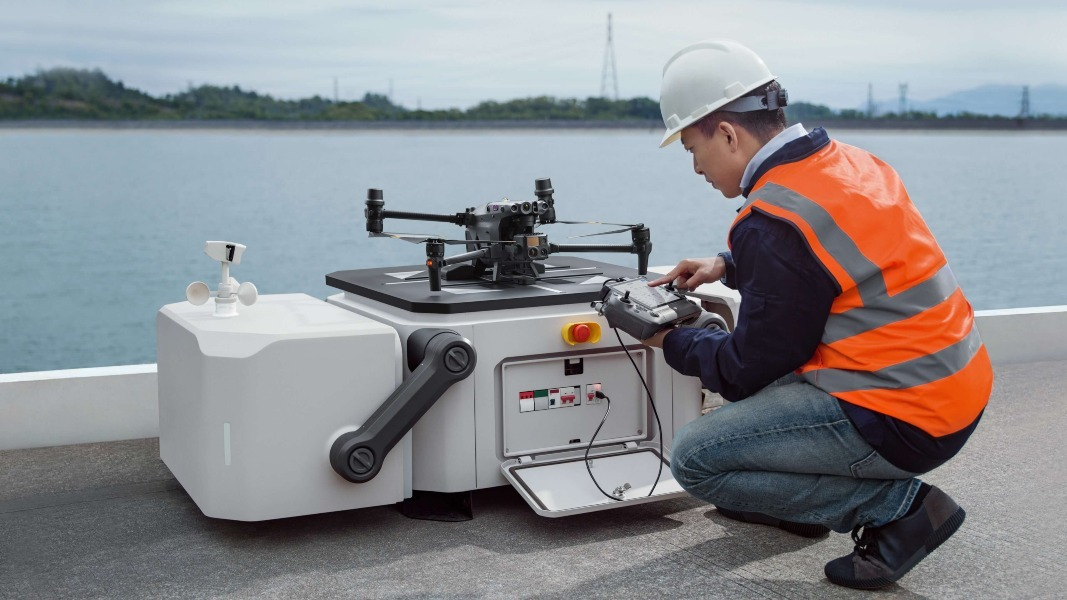
\includegraphics[width=10cm]{pictures/drone_box.jpg}
\centering
\end{figure}

No es justo ver las declaraciones de cuánto se gasta en la adqusición de un nuevo drone en cualquier gobierno. Confío que se puede lograr cosas interesantes con la inversión y realización de buenos productos con la sinergia gobierno-academia. 

\mybox{Ventajas}{green!40}{green!10}{Facilitación de mapeo y seguiridad en tiempo "real".\\
Se puede hacer uso del procesamiento en la nube, y poder sacar el potencial que la Inteligencia Computacional nos puede brindar como el reconocimiento de actividades ilicitas (sólo por mencionar alguna).}

\mybox{Desventajas}{red!40}{red!10}{Autonomía de vuelo y de zonas de inspección.\\
A pesar del despliegue de las redes 5G, los ductos o zonas a vigilar están en zonas no urbanas y fuera de alguna zona de cobertura de red celular}

%------------------------------------------------
\newpage
\subsection{Manupulación de Objetos para trabajos de altura}

El desarrollo acelerado de la tecnología abarca prácticamente todos los campos del saber e impacta una amplia gama de actividades que se llevan a cabo hoy en día (Carpio, 2018). Actualmente existe un progreso asombroso en el aprendizaje automático y la inteligencia artificial, persistiendo la necesidad de desarrollar conjuntos socio-tecnológicos de humanos y máquinas para lograr colectivamente resultados superiores.\\

\begin{figure}[h]
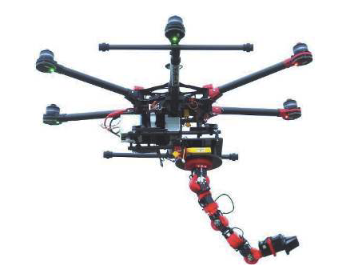
\includegraphics[width=8cm]{pictures/arm_drone.png}
\centering
\end{figure}

\mybox{Ventajas}{green!40}{green!10}{This is a very different box... Well, ok, just the colour.}

\mybox{Desventajas}{red!40}{red!10}{Everything needed to decrypt the drive data is stored on the drive itself. No secret is
  present in the enclosure.}

\newpage
\subsection{Polonización robótica}

%El surgimiento reciente de vehículos aéreos no tripulados (VANTs), concretamente los drones, forman parte de esos avances que ha revolucionado en los últimos años distintos quehaceres relacionados con la comunicación, monitoreo del espacio, seguridad ciudadana, agricultura y tráfico automotor, entre otros. Destacando tecnologías avanzadas como imágenes espectrales, robótica e inteligencia artificial (IA) para derivar el sistema de agricultura tradicional a un sistema de agricultura moderno

Actualmente los problemas derivados del cambio climático y de otras causas más específicas, entre ellas el uso de dispositivos o trampas de insectos en cultivos han impactado directamente la población de insectos fitófagos \href{http://www.scielo.org.pe/scielo.php?pid=S2077-99172020000100061&script=sci_abstract}{(Bravo-Portocarrero et al., 2020)}, y probablemente también de algunos polinizadores. De manera que estos fenómenos, así como sus consecuencias, seguramente sea uno de los desafíos que debe asumir el hombre para mitigar sus impactos.\\

\begin{figure}[h]
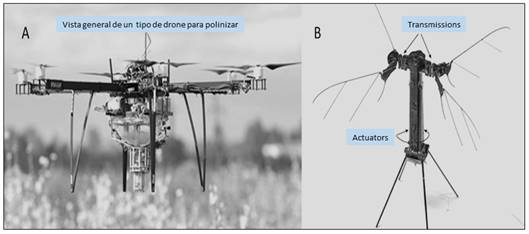
\includegraphics[width=10cm]{pictures/polinizadores.jpg}
\centering
\end{figure}

Ante el panorama descrito, surge una estrategia para aliviar los efectos de la disminución de la polinización natural, específicamente por biopolinizadores como la abeja; es decir, el uso de vehículos aéreos no tripulados tipo drones, de los cuales, ya existen experiencias exitosas de su aplicación en tareas relacionadas con detección de plagas estrés hídrico y análisis de humedad del suelo; pero además, agregan dichos autores, que recientemente diversas empresas diseñan plataformas exclusivas para otras actividades agrícolas específicas, entre ellas, la polinización

\mybox{Ventajas}{green!40}{green!10}{Herramienta potencial en el campo de la agricultura de precisión, particularmente en actividades asociadas a polinización y fertilización. Existe abundante información sobre la aplicación de VANTs en la agricultura, pero en específico para labores de polinización, no es lo mismo.}

\mybox{Desventajas}{red!40}{red!10}{Aunque resulta prematuro hablar de las consecuencias medioambientales de la tecnología en análisis, no deja de preocupar el uso de los VANTs en determinados agroecosistemas, básicamente en aquellos en los que muchas especies de animales desarrollan sus ciclos vitales.\\
  El impacto que los VANTs causarían en la población de polinizadores naturales en los cultivos, los cuales, al observar que estos equipos se acercan hasta ellos pueden generar estrés y otras situaciones que potencialmente afecten su salud.\\
Finalmente, el desarrollo de nuevas investigaciones en torno al uso de drones en actividades de polinización es un reto pendiente, pues de cara al futuro se requiere de mayores conocimientos que conlleven a nuevas readaptaciones de la tecnología VANTs, de forma tal, que sean superadas en el corto tiempo las desventajas y adversidades que hasta ahora implica su uso en la agricultura de precisión
}

\end{document}
